%%%% A summary of basic Markov decision theory.

% Plain and simple
\documentclass{article}

% Format and figure stuff
\usepackage{geometry}
\usepackage{graphicx}
\usepackage{float}
\usepackage[usenames, dvipsnames]{color}

% Text stuff
\usepackage{tikzsymbols}

% Math stuff
\usepackage{mathtools}
\usepackage{mathrsfs}
\usepackage{amsmath}
\usepackage{amssymb}
\usepackage{cancel}
\usepackage{xfrac}
\usepackage{bm}

% Code stuff
\usepackage{listings}
\usepackage{hyperref}

% Page layout
\geometry{top=1in,bottom=1in}
\hyphenpenalty = 10000
\setlength\parindent{0pt}
\setlength{\jot}{10pt}

% Hyperlink format
\hypersetup{colorlinks=true,
            linkcolor=blue,
            filecolor=magenta,
            urlcolor=blue}

% Tab command
\newcommand\tab[1][1cm]{\hspace*{#1}}

% Line command
\newcommand\myline{\noindent\makebox[\linewidth]{\rule{\paperwidth - 2in}{0.4pt}}}

% Code font
\def\code#1{\texttt{#1}}

% Quick colors
\definecolor{stateblue}{rgb}{0, 0, 0.75}
\definecolor{darkgreen}{rgb}{0, 0.5, 0}
\definecolor{orange}{RGB}{180, 60, 0}
\definecolor{purple}{RGB}{200, 0, 200}
\def\green#1{\textcolor{darkgreen}{#1}}
\def\red#1{\textcolor{red}{#1}}
\def\blue#1{\textcolor{stateblue}{#1}}
\def\orange#1{\textcolor{orange}{#1}}
\def\purple#1{\textcolor{purple}{#1}}
\def\black#1{\textcolor{black}{#1}}

% Coordinate system notation
\def\cs#1#2%
  {\mathop{}%
   \mathopen{\vphantom{#2}}^{#1}%
   \kern-\scriptspace%
   #2}

% Custom math symbols - linear algebra
\DeclareMathOperator*{\tr}{\intercal}
\DeclareMathOperator*{\zero}{\underline{0}}
\DeclareMathOperator*{\eye}{\underline{1}}
\newcommand\inv[1]{#1\raisebox{1.15ex}{$\scriptscriptstyle-\!1$}}
\newcommand\pinv[1]{#1\raisebox{1.15ex}{$\scriptscriptstyle\dist\!1$}}

% Custom math symbols - probability
\DeclareMathOperator*{\E}{E}
\DeclareMathOperator*{\cov}{cov}
\DeclareMathOperator*{\dist}{\sim}
\DeclareMathOperator*{\argmin}{arg\,min}
\DeclareMathOperator*{\argmax}{arg\,max}


\begin{document}

%%%%%%%%%%%%%%%%%%%%%%%%%%%%%%%%%%%%%%%%%%%%%%%%% TITLE

\title{\textbf{Markov Decision Processes}\\ \large{A Reasonably Precise Summary}\vspace{-6ex}}
\author{\vspace{-5ex}}
\date{\small{Jason Nezvadovitz -- February 2020}}
\maketitle

%%%%%%%%%%%%%%%%%%%%%%%%%%%%%%%%%%%%%%%%%%%%%%%%% BODY

The purpose of this document is to provide a written, mathematically precise summary of basic Markov decision theory for review. The focus is on axiomatic clarity rather than intuition. I encourage the reader to try explaining each statement intuitively while verifying its consistency.

\vspace{0.2in}
\hrule
\vspace{0.2in}

Declare ``time'': a countable set $\mathbb{T} = \{0, 1, 2, \cdots, n\}$ for some potentially infinite ``horizon'' $n$.\\
Denote a generic element as $t \in \mathbb{T}$.\\

In the most general setting, time can be continuous (uncountable), but we will restrict ourselves to discrete time here to avoid the complications of stochastic calculus.\\

Declare the ``state space'': a set $\mathbb{S}$ of any cardinality. Could be $\mathbb{R}^2$, \{\Smiley,\Cooley,\Winkey\}, whatever.\\
Denote a generic element as $s \in \mathbb{S}$.\\

Declare the ``action space'': a set $\mathbb{A}$ of any cardinality. No restrictions.\\
Denote a generic element as $a \in \mathbb{A}$.\\

We will now build a standard \href{https://en.wikipedia.org/wiki/Probability_space}{probability space}, $\boldsymbol{(}\Omega, \mathcal{F}, P\boldsymbol{)}$.\\

Let the sample space be \ $\Omega = \mathbb{S}^{n+1} \times \mathbb{A}^n \times \mathbb{R}^n$.\\
An individual sample $\omega \in \Omega$ is called a ``trajectory.''\\

Each trajectory consists of an ``initial condition'' $s_0$, and $n$ triplets of the form $(a_t, s_{t+1}, r_{t+1})$ called ``transitions,'' where the $r \in \mathbb{R}$ are called ``rewards.'' I.e.,
\begin{equation*}
\omega = \{s_0, (a_0, s_1, r_1), (a_1, s_2, r_2), \cdots, (a_{n-1}, s_{n}, r_n)\}
\end{equation*}

The event set $\mathcal{F}$ is, as usual, the product sigma-algebra of $\Omega$, using the Borel sigma-algebra for uncountable sets and the power-set sigma-algebra for countable sets.\\

The probability measure $P$ is, as usual, defined in terms of the probability distribution $p$ by sums,
\begin{equation*}
P(B) = \int_B p(\omega)\, d\omega\ \ \forall B \in \mathcal{F},\ \ \text{where}\ \ p(\omega)\geq0\ \ \text{and}\ \ \int_\Omega p(\omega)\,d\omega = 1
\end{equation*}

We declare $p$ to have ``Markovian'' structure, i.e. the following factorization:
\begin{align*}
p(\omega) &= p(s_0, a_0, s_1, r_1, a_1, s_2, r_2, \cdots, a_{n-1}, s_{n}, r_n)\\
&\stackrel{\text{markov}}{=}\ p(s_0) \prod_{t=0}^{n-1} \red{p(a_t|s_t)}\blue{p(s_{t+1}|s_t,a_t)}\green{p(r_{t+1}|s_t,a_t,s_{t+1})}
\end{align*}

where we are using the usual overloaded notation for marginal and conditional distributions,\\
\begin{equation*}
p(x) = \int p(x,y)\,dy\ \ \ \text{and}\ \ \ p(x|y) = \frac{p(x,y)}{p(y)}
\end{equation*}

Practically speaking, the Markov property allows us to completely define high-dimensional trajectory probabilities $p(\omega)$ by specifying just the following lower-dimensional distributions:
\begin{itemize}
  \item The ``initial condition'' $p(s_0)$
  \item The ``\red{policies}'' $p(a_t|s_t)\ \forall t$
  \item The ``\blue{dynamics}'' $p(s_{t+1}|s_t,a_t)\ \forall t$
  \item The ``\green{rewards}'' $p(r_{t+1}|s_t,a_t,s_{t+1})\ \forall t$
\end{itemize}

If, for example, the expression of $p(a_t|s_t)$ does not depend explicitly on the time index $t$, then we say there is just one ``policy'' (nonplural) and that it is ``time-invariant.'' It is often the case that all of the above are time-invariant, and so we really only have one unique policy, one unique dynamic, and one unique reward distribution that are just replicated $n$-times in the factorization of $p(\omega)$.\\

Also, whenever a distribution's form is that of a Dirac-delta, we call it ``deterministic'' instead of ``stochastic.'' It is common for both the policies and rewards to be deterministic. In fact, the reward distribution is often deterministic, time-invariant, and even independent of $s_{t+1}$, meaning that it can be fully specified by a single function $\bar{r}:\mathbb{S}\times\mathbb{A} \to \mathbb{R}$ through,
\begin{equation*}
p(r_{t+1}|s_t,a_t,s_{t+1}) \ \stackrel{\text{commonly}}{=} \ \delta\big{(}r_{t+1} - \bar{r}(s_t, a_t)\big{)}
\end{equation*}

Anyway, the Markov property implies many strong conditional independence statements. E.g.,
\begin{equation*}
p(s_{t+1}|s_t,a_t,s_{t-1},a_{t-1},r_{t-1},s_{t-2},a_{t-2},r_{t-2},\cdots) \stackrel{\text{markov}}{=} p(s_{t+1}|s_t,a_t)
\end{equation*}

These relationships can be depicted succinctly via a \href{https://en.wikipedia.org/wiki/Bayesian_network}{Bayesian graph} over the convenience random variables \ ${s_t}(\omega) = s_t$, \ ${a_t}(\omega) = a_t$, \ and \ ${r_t}(\omega) = r_t$.
\begin{center}
  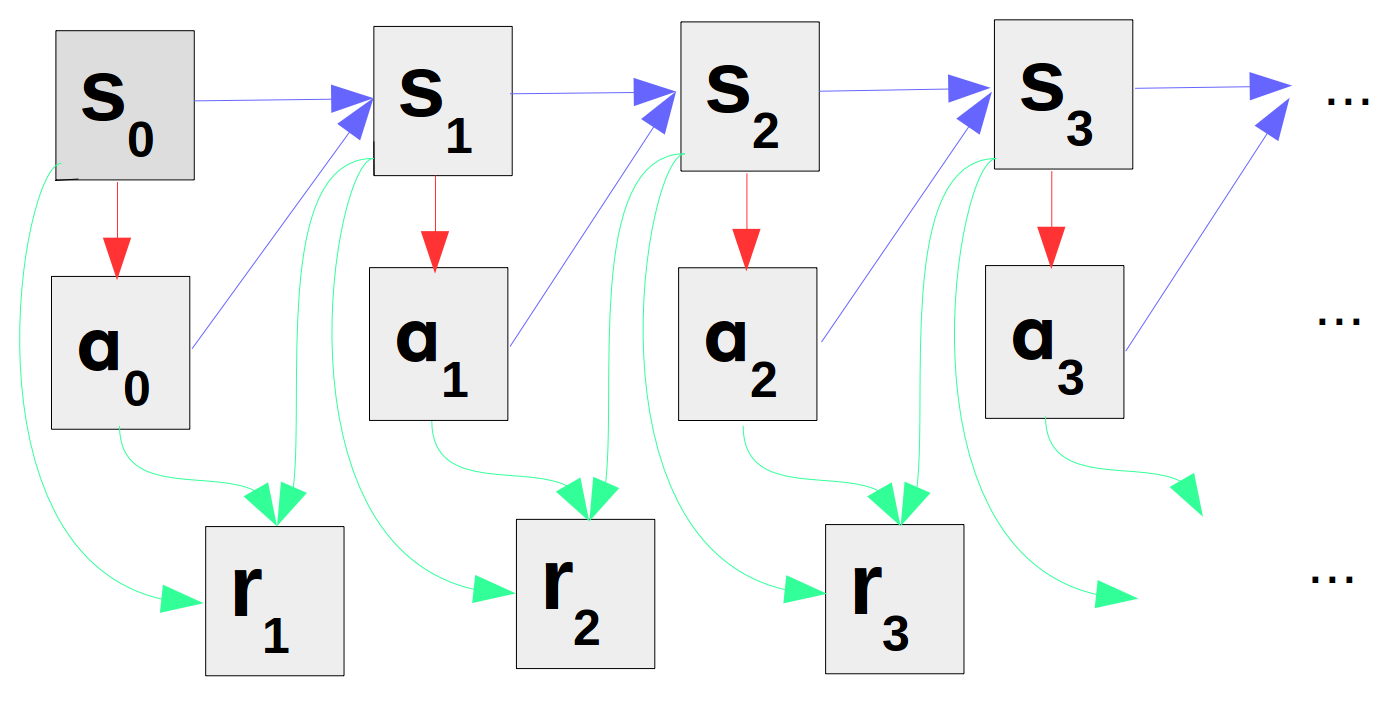
\includegraphics[width=\linewidth-1.5in]{include/bayesgraph.png}
\end{center}

This temporally ``chained'' structure models the idea that ``given the present, the future is independent of the past'' and constitutes the entirety of a ``Markov decision process'' (MDP). Specifically, if we define the random variable $\omega_t$ to be the elements of a trajectory for times $\tau \geq t$ (``the future''),
\begin{equation*}
\omega_t = \{s_t, (a_t, s_{t+1}, r_{t+1}), (a_{t+1}, s_{t+2}, r_{t+2}), \cdots, (a_{n-1}, s_{n}, r_n)\} \ \in \ \Omega_t = \mathbb{S}^{n-t+1} \times \mathbb{A}^{n-t} \times \mathbb{R}^{n-t}
\end{equation*}

we see from the Bayesian graph that $\omega_t$ is disconnected from ``the past'' by conditioning on $s_t$,
\begin{equation*}
p(\omega_t|s_t) = \cancel{\frac{p(s_t)}{p(s_t)}}\prod_{\tau=t}^{n-1} p(a_\tau|s_\tau)p(s_{\tau+1}|s_\tau,a_\tau)p(r_{\tau+1}|s_\tau,a_\tau,s_{\tau+1})
\end{equation*}

We now define the ``total (discounted) reward from $t$'' to be a random variable that assesses the goodness of a sample of our MDP starting from time $t$ by summing up the remaining rewards,
\begin{align*}
G_t(\omega_t) &= r_{t+1} + \gamma r_{t+2} + \gamma^2 r_{t+3} + \cdots + \gamma^{n-t-1} r_n\\
&= \sum_{\tau=t}^{n-1} \gamma^{\tau-t} r_{\tau+1}
\end{align*}

where $\gamma \in [0,1]$ is called the ``discount factor,'' used both to enforce the convergence of this sum (if $n \to \infty$) and to express that future rewards are less valuable than sooner rewards.\\

Total reward provokes an optimization problem: we want to choose the best possible policy distribution $p(a_t|s_t)$. To clarify, the ``decision'' in ``Markov decision process'' is really deciding the distribution from which actions will be sampled (the policy). If the policy depends only on time (ignoring the actual value of $s_t$) we call it ``open-loop'' or a ``plan,'' while if it depends on $s_t$ in any way we call it ``closed-loop.'' If the policy is deterministic and time-invariant, then it can be fully specified by a single function $\mathbb{S} \mapsto \mathbb{A}$ that is interpreted classically as a decision-making rule.\\

We will denote our choice as $\pi(a_t|s_t)$, and to emphasize that we have plugged-in our choice, we will use $\pi$ as a subscript on probability densities and statistics. For example,
\begin{equation*}
p_{\orange{\pi}}(\omega) = p(s_0) \prod_{t=0}^{n-1} \orange{\pi(a_t|s_t)}p(s_{t+1}|s_t,a_t)p(r_{t+1}|s_t,a_t,s_{t+1})
\end{equation*}

But what does ``best'' mean with respect to a random variable like $G_t$? We choose to optimize a statistic of $G_t$. Namely, a conditional expectation called the ``value function,''
\begin{align*}
V_\pi(s_t) &= E_\pi(G_t | s_t)\\
&= \int_{\Omega_t} G_t(\omega_t) p_\pi(\omega_t|s_t)\,d\omega_t\\
&= \int_{\Omega_t} \sum_{\tau=t}^{n-1} \Big{(}\gamma^{\tau-t} r_{\tau+1}\Big{)} \prod_{\tau=t}^{n-1} \Big{(}\pi(a_\tau|s_\tau)p(s_{\tau+1}|s_\tau,a_\tau)p(r_{\tau+1}|s_\tau,a_\tau,s_{\tau+1})\Big{)} \,d\omega_t
\end{align*}

I.e., $V_\pi(s_t)$ is the expected total reward acquired for starting from state $s$ at time $t$ and acting according to policy $\pi$. Our objective then is to find the optimal policy $\pi^*$ that satisfies,
\begin{equation*}
V_{\pi^*}(s_t) \geq V_{\pi}(s_t)\ \forall s_t
\end{equation*}

The existence of such a $\pi^*$ is guaranteed by Bellman's Principle\ldots

\vspace{0.3in}

- Bellman equation (derive recursion, dynamic programming principle, robber problem example, LQR example)\\

- Value iteration (contraction mapping, fixed-point iteration, example with small S and use markov diagram)\\

- Q-learning (k-step value functions, transition monte carlo, example with same small S)\\

- Approximation (linear basis, deep nets, experience replay, $|S|$ vs $V$ smoothness, example with large S)\\

- Policy gradient (analytical derivative, trajectory monte carlo)\\

- Further topics (POMDP / HMM, game theory / multiagent)


% One possible approach to this optimization is to parameterize the policy as $\pi_\theta(a_t|s_t;\theta)$, express the analytical gradient of $V_\pi(s_t)$ with respect to $\theta$, and then numerically evaluate the remaining intractable integral by monte-carlo. This approach is called ``policy gradient'' or sometimes ``direct policy search.'' However, there is a recursion that yields a more elegant (my opinion) approach known as ``dynamic programming'' or ``Bellman's principle.''\\

% We find the following recursion,
% \begin{align*}
% G_t &= r_{t+1} + \sum_{i=0}^{n-1} \gamma^{(i+1)} r_{t+1+(i+1)}\\
% &= r_{t+1} + \gamma G_{t+1}
% \end{align*}

% We find the following recursion for the value function (invoking the total-expectation identity),
% \begin{align*}
% V_\pi(s_t) &= E_\pi(r_{t+1} + \gamma G_{t+1} | s_t)\\
% &= E_\pi(r_{t+1}|s_t) + \gamma E_\pi(G_{t+1} | s_t)\\
% &= E_\pi(r_{t+1}|s_t) + \gamma E_\pi\big{(}E_\pi(G_{t+1}|s_{t+1},s_{t}) | s_t\big{)}\\
% &= E_\pi(r_{t+1}|s_t) + \gamma E_\pi\big{(}E_\pi(G_{t+1}|s_{t+1}) | s_t\big{)}\\
% &= E_\pi(r_{t+1}|s_t) + \gamma E_\pi\big{(}V_\pi(s_{t+1}) | s_t\big{)}\\
% \end{align*}

% &= E_\pi(r_{t+1} + \gamma V_\pi(s_{t+1}) | s_t)
% \end{align*}

% Defining the ``transition operator,''
% $$
% T_\pi f(s_t,\cdots) = E_\pi\big{(}f(s_{t+1},\cdots)|s_t\big{)}
% $$

% we have,
% $$
% V_\pi(s_t) = T_\pi\big{(}r_{t} + \gamma V_\pi(s_t)\big{)}
% $$

% Bellman's principle of optimality says that the optimal action now is that which maximizes the immediate reward plus the optimal total reward we can \textit{expect} to get from the state this action puts us in. Applying this principle:
% $$
% V_{\pi^*}(s_t) = \max_{a} \Big{(} T_a\big{(}r_{t} + \gamma V_{\pi^*}(s_t)\big{)} \Big{)} \implies V_{\pi^*}(s_t) \geq V_{\pi}(s_t)\ \forall s_t
% $$

% where,
% $$
% T_a f(s_t,\cdots) = E\big{(}f(s_{t+1},\cdots)|s_t,a_t=a\big{)}
% $$\\

% The general Bellman recursion:
% $$
% V_\pi(s_t) = E_\pi\big{(}r_{t+1} + \gamma V_\pi(s_{t+1}) \big{|} s_t\big{)}
% $$

% \textit{The} Bellman Equation
% $$
% V_{\pi^*}(s_t) = \max_a\Big{(}E\big{(}r_{t+1} + \gamma V_{\pi^*}(s_{t+1}) \big{|} s_t, a_t=a\big{)}\Big{)}
% $$

%%%%%%%%%%%%%%%%%%%%%%%%%%%%%%%%%%%%%%%%%%%%%%%%%

\end{document}
